\documentclass[10pt]{beamer}
\usetheme{jambro}
\graphicspath{{./graphics/}}

% Authors/institutes/date/etc
%--------------------------------
\title[]{Jambro Beamer Template}
\author[]{Ambrogio Cesa-Bianchi}
\date{\today}

\begin{document}

%=============================================================
\begin{frame}[plain]
    \titlepage{
        \begin{center}
            \begin{minipage}{0.8\textwidth}
                \centering
                \color{title!80}{\scriptsize *The Usual Disclaimer Applies}
            \end{minipage}
    \end{center}}
\end{frame}
%.......................................................
\begin{flushleft}
    \underline{\textbf{Notes}}\setlength{\parskip}{.15cm}\notesize\newline\par
    These are some speaking notes on the title slide \par
    And some more 
\end{flushleft}

%=============================================================
\begin{frame}
    \frametitle{Table of Contents}
    \tableofcontents
\end{frame}
%.......................................................
\begin{flushleft}
    \underline{\textbf{Notes}}\setlength{\parskip}{.15cm}\notesize\newline\par
    These are some speaking notes on the title slide \par
    And some more 
\end{flushleft}

%=============================================================
\section{Introduction}
\begin{frame}{Jambro Beamer Theme}
    \small
    \begin{itemize}
        \item Jambro is a Beamer theme with a strong focus on clarity and readability:
        \begin{itemize}
            \item Clean, minimalist layout \smallskip
            \item Subtle color palette \smallskip
            \item Modern typography \smallskip
            \item Spacious design ideal for academic or policy presentations \bigskip
        \end{itemize}
        \item Getting started:
        \begin{itemize}
            \item After the usual \texttt{\textbackslash documentclass\{beamer\}}, load the theme with \texttt{\textbackslash usetheme\{jambro\}} \smallskip
            \item The file \texttt{beamerthemejambro.sty} must be in the same folder as your Beamer presentation
        \end{itemize}
    \end{itemize}
\end{frame}
%.......................................................
\begin{flushleft}
    \underline{\textbf{Notes}}\setlength{\parskip}{.15cm}\notesize\newline\par
\end{flushleft}

%=============================================================
\section{Arrows \& Handwriting}
\begin{frame}
    \begin{eqnarray*}
        &\text{{\huge \textbf{Arrows \& Handwriting}}}\\
    \end{eqnarray*}
\end{frame}
%.......................................................
\begin{flushleft}
    \underline{\textbf{Notes}}\setlength{\parskip}{.15cm}\notesize\newline\par
\end{flushleft}

%=============================================================
\begin{frame}[t,fragile]
    {Arrows and handwritten notes}\bigskip
    \begin{itemize}
        \item The theme embeds a way to introduce handwritten notes using arrows \bigskip\medskip
        \item Imagine you want to clarify something about \marker{node1}{$x$} \bigskip\medskip\pause
        \item The theme allows to add arrows and handwritten notes using \texttt{\textbackslash hand} command and Tikz \medskip
        \begin{itemize}
            \item Use command \texttt{\textbackslash marker\{\textit{mylabel}\}\{\textit{text}\}} to anchor the arrow \medskip
            \item Then use standard Tikz syntax \par\medskip
            \hspace{-2cm}
            \begin{minipage}{\textwidth}
                \scriptsize
                \begin{verbatim}
                    \begin{tikzpicture}[tpstyle]
                        \draw[arrow,->] ([yshift=2pt]node1.north east) to[bend left] +(0.7,+0.3) %
                        node[anchor=west] {\hand A comment from the north};
                    \end{tikzpicture}		
                \end{verbatim}
            \end{minipage}           
            \begin{tikzpicture}[tpstyle]
                \draw[arrow,->] ([yshift=2pt]node1.north east) to[bend left] +(0.7,+0.3) node[anchor=west] {\hand A comment from the north};
            \end{tikzpicture}		
        \end{itemize}
    \end{itemize}
\end{frame}
%.......................................................
\begin{flushleft}
    \underline{\textbf{Notes}}\setlength{\parskip}{.15cm}\notesize\newline\par
\end{flushleft}

%=============================================================
\begin{frame}[t]
    {Arrows and handwritten notes}\bigskip
    \begin{itemize}
        \item The theme embeds a way to introduce handwritten notes using arrows \bigskip\medskip
        \item Imagine you want to clarify something about \marker{node1}{$x$} \bigskip\medskip
        \item The theme allows to add arrows and handwritten notes using \texttt{\textbackslash hand} command and Tikz \medskip
        \begin{itemize}
            \item Arrows can start from different cardinal points 
            \begin{tikzpicture}[tpstyle]
                \draw[arrow,->] ([yshift=2pt]node1.north east) to[bend left] +(0.7,+0.3) node[anchor=west] {\hand A comment from the north};
                \draw[arrow,->] ([yshift=-2pt]node1.south) to[bend right] +(1.6,-0.2) node[anchor=west] {\hand A comment from the south};
            \end{tikzpicture}	
        \end{itemize}
    \end{itemize}
\end{frame}
%.......................................................
\begin{flushleft}
    \underline{\textbf{Notes}}\setlength{\parskip}{.15cm}\notesize\newline\par
\end{flushleft}

%=============================================================
\begin{frame}[t]
    {Arrows and handwritten notes}\bigskip
    \begin{itemize}
        \item The theme embeds a way to introduce handwritten notes using arrows \bigskip\medskip
        \item Imagine you want to clarify something about \marker{node1}{$x$} \bigskip\medskip
        \item The theme allows to add arrows and handwritten notes using \texttt{\textbackslash hand} command and Tikz \medskip
        \begin{itemize}
            \item Arrows can start from different cardinal points... \medskip
            \item ...have different colors and opacity... \medskip
            \begin{tikzpicture}[tpstyle]
                \draw[arrow,->,brick,opacity=0.5] ([yshift=2pt]node1.north east) to[bend left] +(0.7,+0.3) node[brick,anchor=west,opacity=0.5] {\hand A comment from the north};
                \draw[arrow,->,brick] ([yshift=-2pt]node1.south) to[bend right] +(1.6,-0.2) node[brick,anchor=west] {\hand A comment from the south};
            \end{tikzpicture}	
        \end{itemize}
    \end{itemize}
\end{frame}
%.......................................................
\begin{flushleft}
    \underline{\textbf{Notes}}\setlength{\parskip}{.15cm}\notesize\newline\par
\end{flushleft}

%=============================================================
\begin{frame}[t]
    {Arrows and handwritten notes}\bigskip
    \begin{itemize}
        \item The theme embeds a way to introduce handwritten notes using arrows \bigskip\medskip
        \item Imagine you want to clarify something about \marker{node1}{$x$} \bigskip\medskip
        \item The theme allows to add arrows and handwritten notes using \texttt{\textbackslash hand} command and Tikz \medskip
        \begin{itemize}
            \item Arrows can start from different cardinal points... \medskip
            \item ...have different colors and opacity... \medskip
            \item ...have wiggles....
            \begin{tikzpicture}[tpstyle]
                \draw[arrow,->,brick,opacity=0.5] ([yshift=2pt]node1.north east) to[bend left] +(0.7,+0.3) node[brick,anchor=west,opacity=0.5] {\small{\hand A comment from the north}};
                \draw[snake,->,brick] ([yshift=-2pt]node1.south) to[bend right] +(1.6,-0.2) node[brick,anchor=west] {\small{\hand A comment from the south}};
            \end{tikzpicture}	
        \end{itemize}
    \end{itemize}
\end{frame}
%.......................................................
\begin{flushleft}
    \underline{\textbf{Notes}}\setlength{\parskip}{.15cm}\notesize\newline\par
\end{flushleft}

%=============================================================
\begin{frame}[t]
    {Arrows and handwritten notes}\bigskip
    \begin{itemize}
        \item The theme embeds a way to introduce handwritten notes using arrows \bigskip\medskip
        \item Imagine you want to clarify something about \marker{node1}{$x$} \bigskip\medskip
        \item The theme allows to add arrows and handwritten notes using \texttt{\textbackslash hand} command and Tikz \medskip
        \begin{itemize}
            \item Arrows can start from different cardinal points... \medskip
            \item ...have different colors and opacity... \medskip
            \item ...have wiggles... \medskip
            \item ...be bidirectional or adirectional
            \begin{tikzpicture}[tpstyle]
                \draw[arrow,brick,opacity=0.5] ([yshift=2pt]node1.north east) to[bend left] +(0.7,+0.3) node[brick,anchor=west,opacity=0.5] {\hand A comment from the north};
                \draw[snake,<->,brick] ([yshift=-2pt]node1.south) to[bend right] +(1.6,-0.2) node[brick,anchor=west] {\hand A comment from the south};
            \end{tikzpicture}	
        \end{itemize}
    \end{itemize}
\end{frame}
%.......................................................
\begin{flushleft}
    \underline{\textbf{Notes}}\setlength{\parskip}{.15cm}\notesize\newline\par
\end{flushleft}

%=============================================================
\begin{frame}[t]
    {Handwritten notes to figures}
    \begin{itemize}
        \item Add notes to figures using the \texttt{tikzpicture} environment
    \end{itemize}
    \begin{center}
        \begin{minipage}[b]{.6\textwidth}
            \begin{tikzpicture}
                \node[inner sep=0] (image) at (0,0) {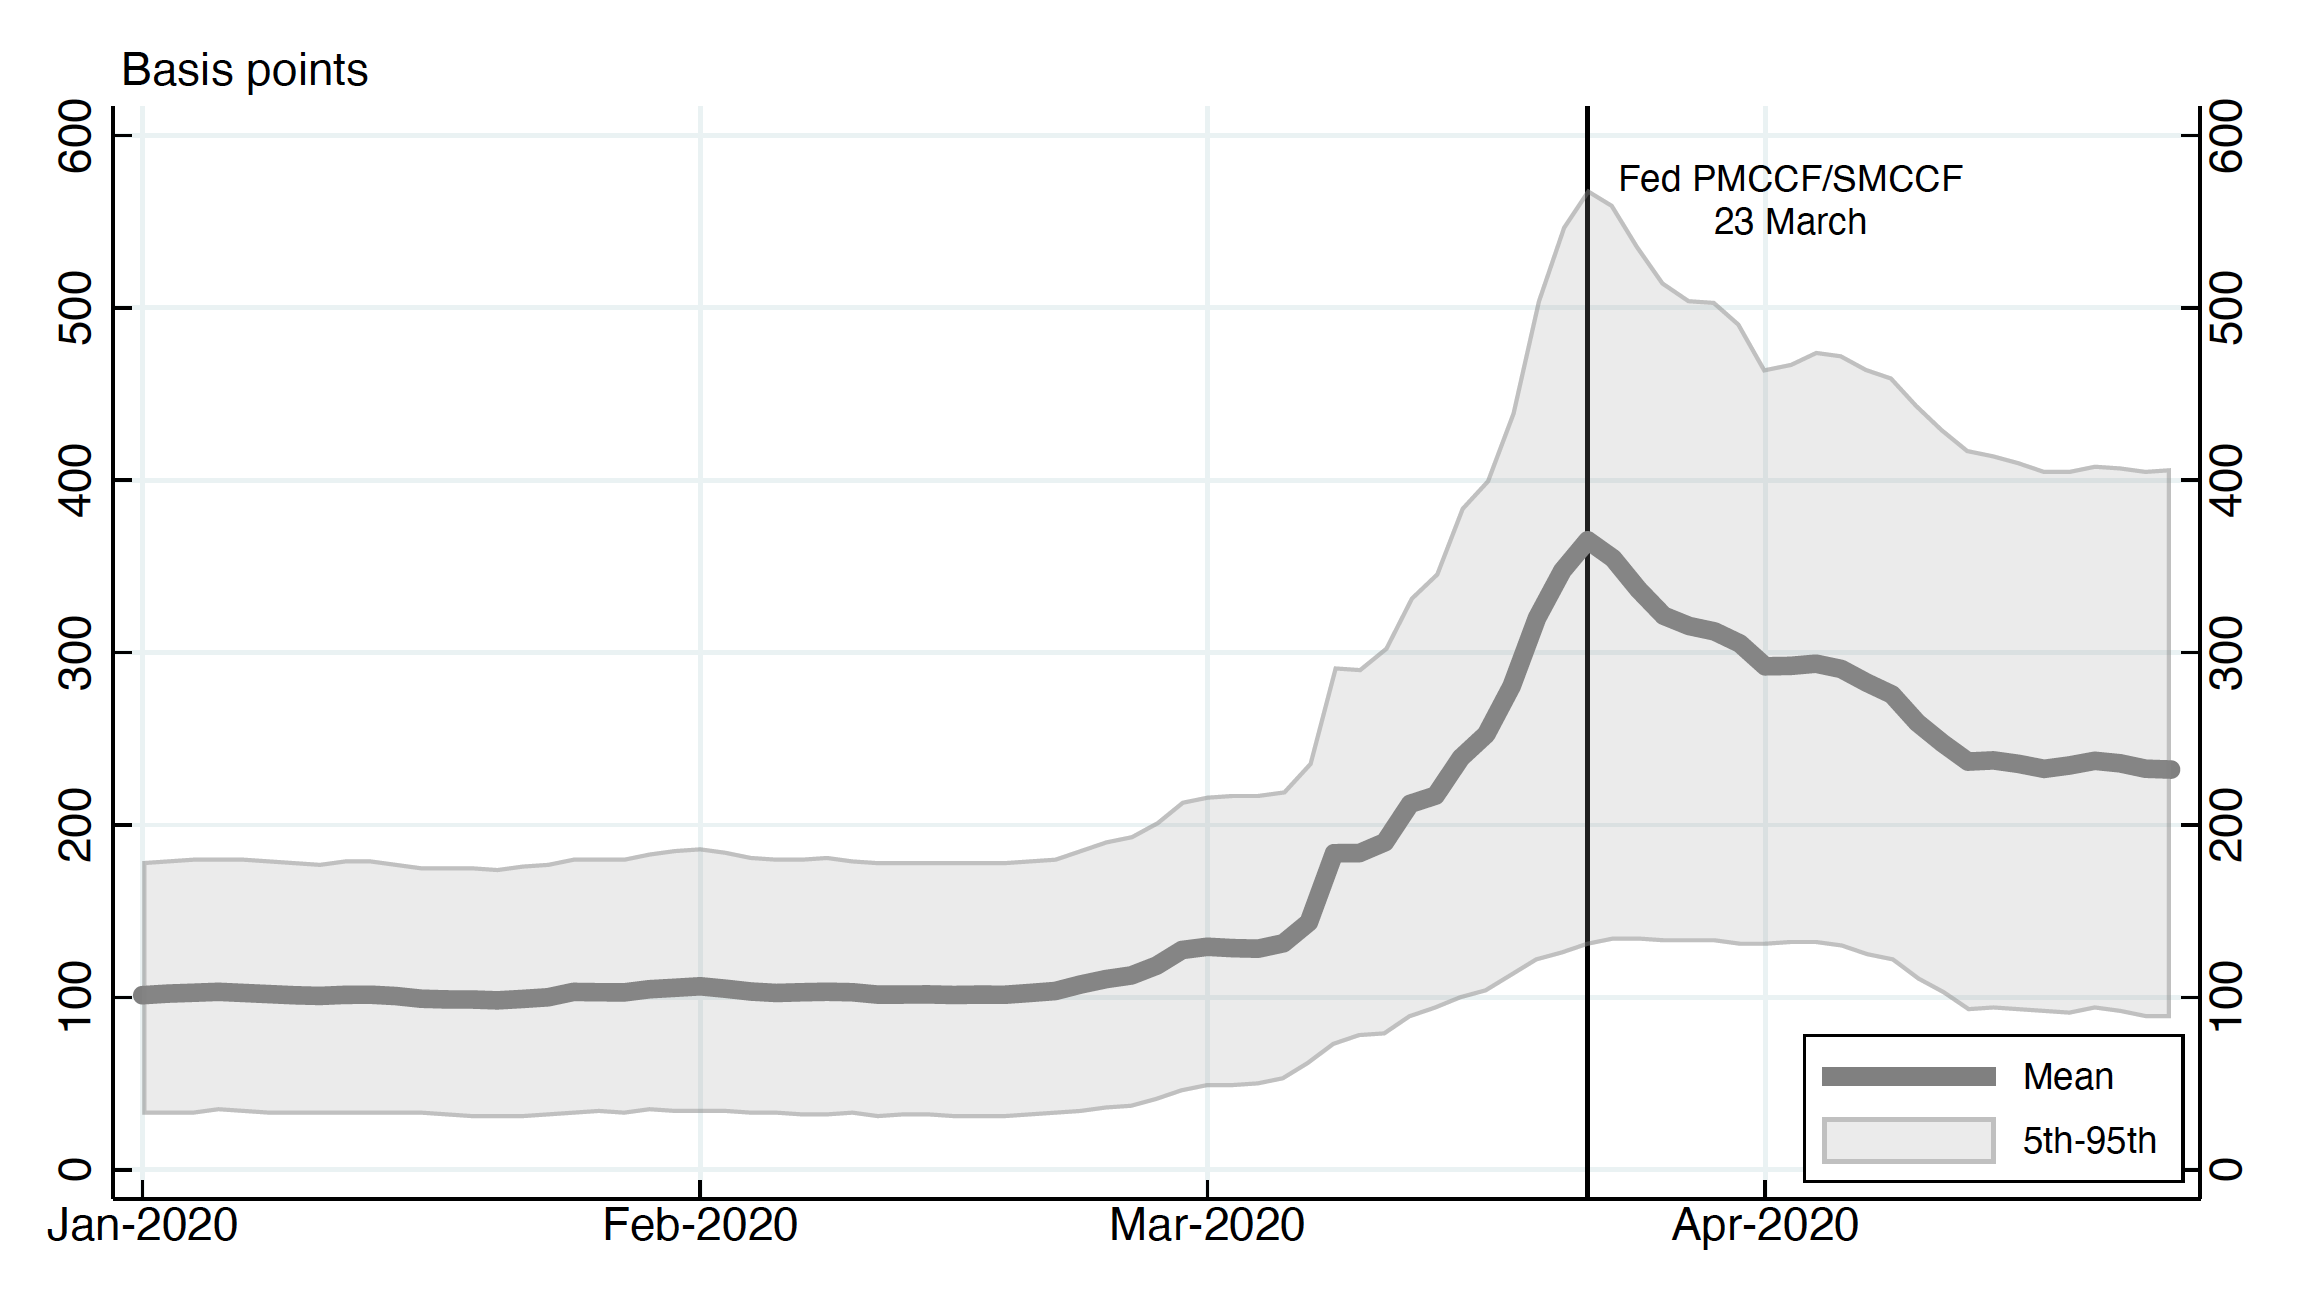
\includegraphics[width=\textwidth]{figure}};
                \draw[arrow,->,opacity=1] (1,0.4) to[bend right] +(-1,+0.9) node[anchor=east,opacity=1] {\normalsize{\hand - One comment}};
                \draw[arrow,->,opacity=1,brick] (0.8,0.4) to[bend right] +(-0.8,-0.6)  node[anchor=east,opacity=1,brick] {\normalsize{\hand - Another comment}};
            \end{tikzpicture}
            \tiny{{\scshape Note}. \ Global average of investment grade corporate bond spreads (option-adjusted) weighted by bonds face value, together with 5th and 95th percentile of the full distribution. Source: ICE BoA ML.} 
        \end{minipage}
    \end{center}
\end{frame}	
%.......................................................
\begin{flushleft}
    \underline{\textbf{Notes}}\setlength{\parskip}{.15cm}\notesize\newline\par
\end{flushleft}

%=============================================================
\begin{frame}[t]
    {Handwritten notes to figures}
    \begin{itemize}
        \item Add shaded areas on top of figures with the \texttt{tikzpicture} environment
    \end{itemize}
    \begin{center}
        \begin{minipage}[b]{.6\textwidth}
            \begin{tikzpicture}
                \node[inner sep=0] (image) at (0,0) {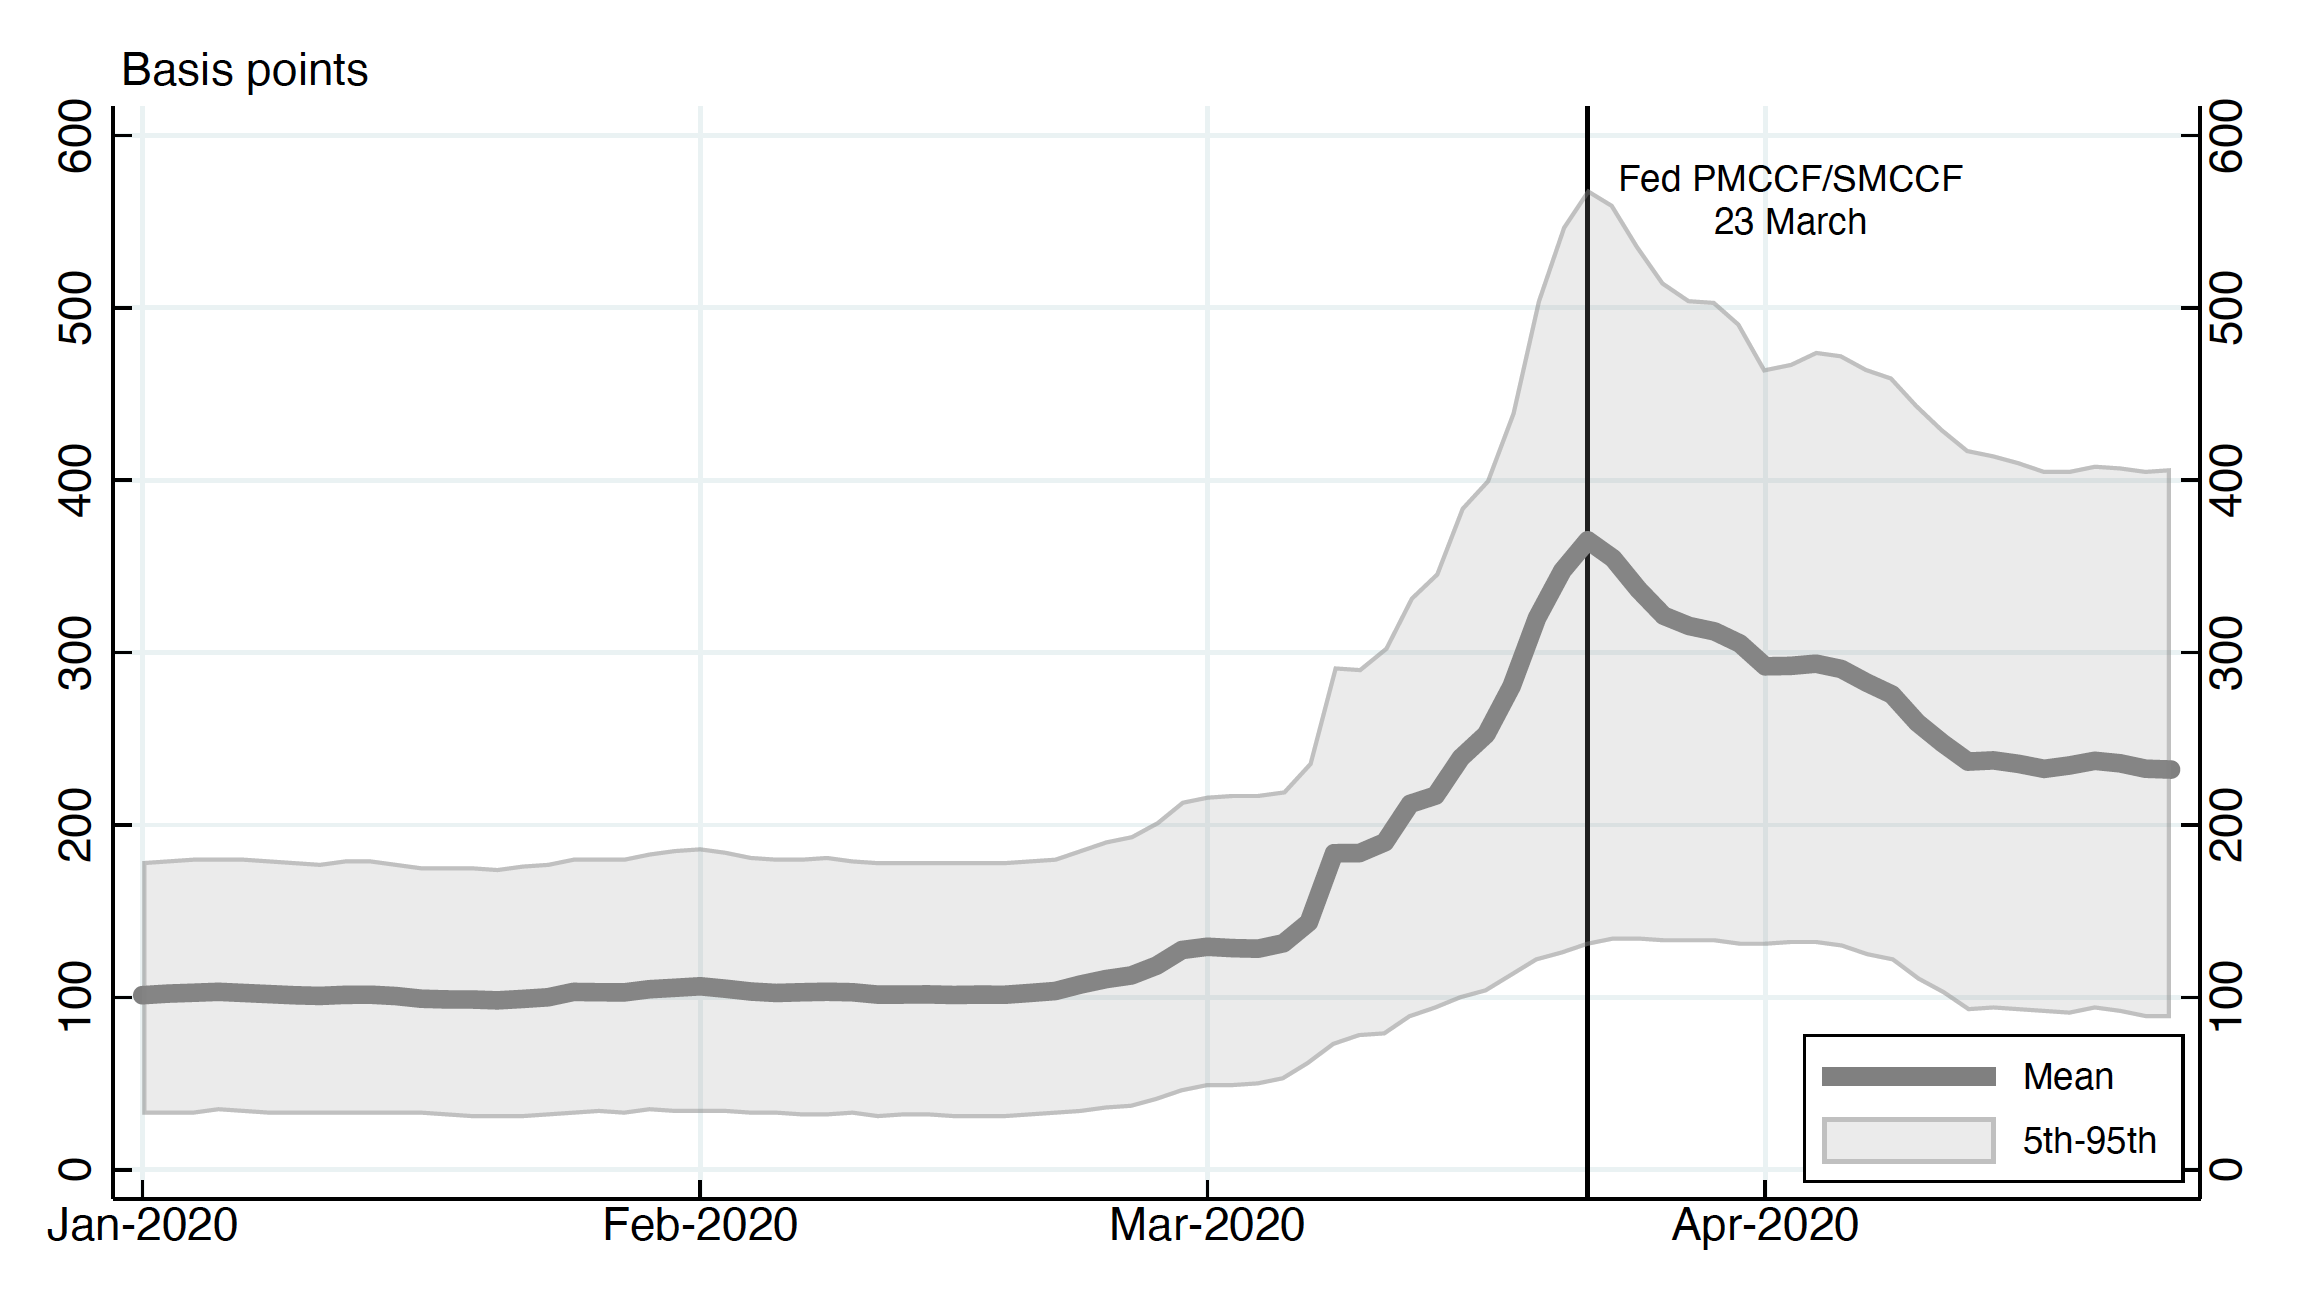
\includegraphics[width=\textwidth]{figure}};
                \draw[arrow,->,opacity=1] (1,0.4) to[bend right] +(-1,+0.9) node[anchor=east,opacity=1] {\normalsize{\hand - One comment}};
                \draw[arrow,->,opacity=1,brick] (0.8,0.4) to[bend right] +(-0.8,-0.6)  node[anchor=east,opacity=1,brick] {\normalsize{\hand - Another comment}};
                \node[rectangle,fill=gold,opacity=0.2,rounded corners=.1cm,minimum width=2cm,minimum height = 5cm] at (0.9,0) {};
            \end{tikzpicture}
            \tiny{{\scshape Note}. \ Global average of investment grade corporate bond spreads (option-adjusted) weighted by bonds face value, together with 5th and 95th percentile of the full distribution. Source: ICE BoA ML.} 
        \end{minipage}
    \end{center}
\end{frame}	
%.......................................................
\begin{flushleft}
    \underline{\textbf{Notes}}\setlength{\parskip}{.15cm}\notesize\newline\par
\end{flushleft}

%=============================================================
\section{Highlighting, Underlying \& Boxing}
\begin{frame}
    \begin{eqnarray*}
        &\text{{\huge \textbf{Highlighting, Underlying}}}\\
        &\text{{\huge \textbf{\& Boxing}}}\\
    \end{eqnarray*}
\end{frame}
%.......................................................
\begin{flushleft}
    \underline{\textbf{Notes}}\setlength{\parskip}{.15cm}\notesize\newline\par
\end{flushleft}

%=============================================================
\begin{frame}
    {Highlighting}
    \begin{itemize}
        \item \stabilo{Highlight text} with the \texttt{\textbackslash stabilo\{\textit{text}\}} command  \medskip
        \begin{itemize}
            \item Can also highlight with a \stabilo[blue_light]{custom color} too using \texttt{\textbackslash stabilo[\textit{mycolor}]\{\textit{text}\}}\bigskip\bigskip
        \end{itemize}
        \item Or \lapis{underline text} using the pencil-like \texttt{\textbackslash lapis\{\textit{text}\}} command \medskip
        \begin{itemize}
            \item Can also highlight with a \lapis[blue_light]{custom color} \ too using \texttt{\textbackslash stabilo[\textit{mycolor}]\{\textit{text}\}}\bigskip\bigskip
        \end{itemize}
        \item You have more control using Tikz directly, for example \medskip
        \begin{itemize}
            \item \tikz[tstyle]{\node[nstyle](node2){Highlight text with a thinner pencil}} (see TEX file for code)
            \begin{tikzpicture}[tpstyle]
                \draw[pencil,line width=0.02cm] ([yshift=-2pt]node2.south west) to ([yshift=-2pt]node2.south east);			
            \end{tikzpicture}  \bigskip
        \end{itemize}
    \end{itemize}
\end{frame}
%.......................................................
\begin{flushleft}
    \underline{\textbf{Notes}}\setlength{\parskip}{.15cm}\notesize\newline\par
\end{flushleft}

%=============================================================
\begin{frame}
    {Boxing text or variables in equations}
    \begin{itemize}
        \item Highlight text with a \lapisbox{pencil-like box effect} using the \texttt{\textbackslash lapisbox\{\textit{text}\}} command  \bigskip\bigskip
        \pause
        \item Can also highlight objects in equations, as well as set colors and labels with \texttt{\textbackslash lapisbox[color=\textit{mycolor},label=\textit{mylabel}]\{\textit{text}\}} \medskip
        \begin{equation*}
            y_{t} = \alpha + \lapisbox[color=tomato,label=box1]{$\beta x_t$} + u_{t} 
        \end{equation*}
        \smallskip\pause
        \item Labels allow to add arrows and comments as before
        \begin{tikzpicture}[tpstyle]
            \draw[arrow,->,tomato!80] ([yshift=-2pt]box1.south east) to[bend right] +(+0.7,-0.5) node[anchor=west,opacity=1,tomato] {\hand A comment from south east};
        \end{tikzpicture}
    \end{itemize}
\end{frame}
%.......................................................
\begin{flushleft}
    \underline{\textbf{Notes}}\setlength{\parskip}{.15cm}\notesize\newline\par
\end{flushleft}

%=============================================================
\begin{frame}
    {Boxing numbers in a table}
    \begin{itemize}
        \item \texttt{lapisbox} can be used to highlight numbers in tables, too \bigskip
    \end{itemize}
    \begin{table}[th]
        \centering%
        \begin{minipage}[b]{.6\textwidth}
            \vspace{.2cm}\tablesize
            \begin{tabularx}{\textwidth}{lY}
                \toprule
                Dep. Variable: spread ($\Delta cs_{ij}$) 	& (1)\\
                \midrule
                & {Baseline Specification} \\
                \midrule
                \rowcolor{gray!10} Coeff. ($\beta_1$) 		&  \lapisbox[color=tomato,label=box1]{21.15***} \\
                &   (7.35) \\
                \midrule
                \rowcolor{gray!10} Double clustering 		& Yes \\
                Time-sector FE 												& No \\
                \rowcolor{gray!10} R-squared 					& 0.034 \\
                Observations 												& 285,794 \\\bottomrule
            \end{tabularx}\vspace{.2cm}\newline
            \tiny{{\scshape Note.} Standard errors (reported in parentheses) are clustered two-way, at the firm level and time level. The asterisks denote statistical significance (*** for $p<0.01$, ** for $p<0.05$, * for $p<0.1$).\newline}%
            \label{tab:label}%
        \end{minipage}
    \end{table}
    \begin{tikzpicture}[tpstyle]
        \draw[arrow,->,tomato] ([xshift=2pt]box1.east) to[bend left] +(+0.7,0) node[anchor=west,opacity=1,tomato] {\hand \small This is a large estimate!};
    \end{tikzpicture}
\end{frame}
%.......................................................
\begin{flushleft}
    \underline{\textbf{Notes}}\setlength{\parskip}{.15cm}\notesize\newline\par
\end{flushleft}

%=============================================================
\section[Options]{Theme's Options}
\begin{frame}
    \begin{eqnarray*}
        &\text{{\huge \textbf{Theme's Options}}}\\
    \end{eqnarray*}
\end{frame}
%.......................................................
\begin{flushleft}
    \underline{\textbf{Notes}}\setlength{\parskip}{.15cm}\notesize\newline\par
\end{flushleft}

%=============================================================
\begin{frame}
    {Theme's options}
    \begin{itemize}
        \item The theme comes with a few options to be specified in the \texttt{\textbackslash documentclass[\textit{option}]\{beamer\}} command \medskip
        \begin{itemize}
            \item \texttt{light}: uses Fira light as a default font\medskip
            \item \texttt{roboto}: changes the default font to Roboto\medskip
            \item \texttt{cabin}: changes the default font to Cabin\medskip
            \item \texttt{night}: switches to night mode colors \medskip
            \item \texttt{red}: switches the main color of the theme from blue to red (this option is overrun by \texttt{night})\medskip
            \item \texttt{3to2}: switches the aspect ratio from 16:9 to 3:2\medskip
            \item \texttt{shownotes}: show notes to the slides \medskip
            \item \texttt{handout}: make handouts with 2x1 slides (portrait). Useful in combination with \texttt{shownotes}\medskip
            \item \texttt{onesec}: visualize only one section at the time in footline (default is all of them)
        \end{itemize}
    \end{itemize}
\end{frame}
%.......................................................
\begin{flushleft}
    \underline{\textbf{Notes}}\setlength{\parskip}{.15cm}\notesize\newline\par
\end{flushleft}

%=============================================================
\begin{frame}
    {Theme's options}
    \begin{itemize}
        \item Set \texttt{light} option for fira font (baseline) in light format 
    \end{itemize}
    \begin{center}
        \begin{minipage}[b]{.6\textwidth}
            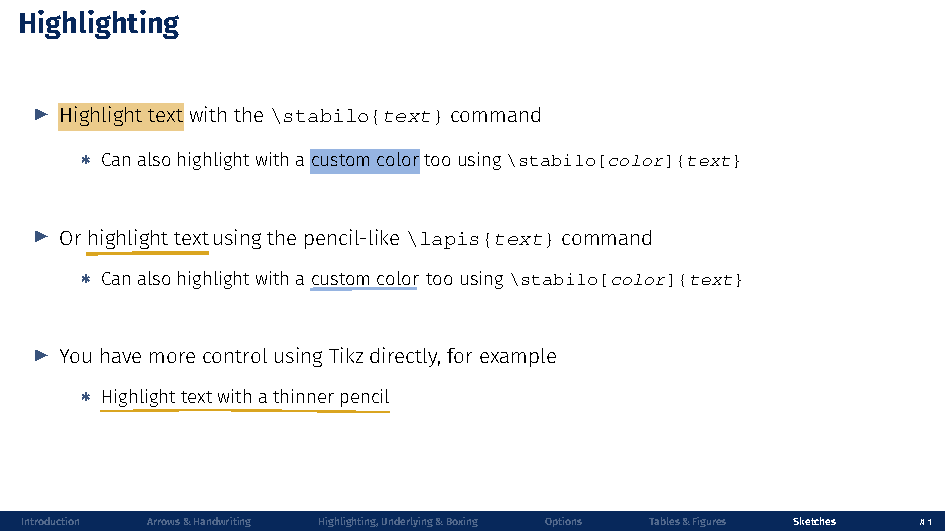
\includegraphics[width=\textwidth]{light}
        \end{minipage}
    \end{center}
\end{frame}
%.......................................................
\begin{flushleft}
    \underline{\textbf{Notes}}\setlength{\parskip}{.15cm}\notesize\newline\par
\end{flushleft}

%=============================================================
\begin{frame}
    {Theme's options}
    \begin{itemize}
        \item Set \texttt{roboto} option for roboto font 
    \end{itemize}
    \begin{center}
        \begin{minipage}[b]{.6\textwidth}
            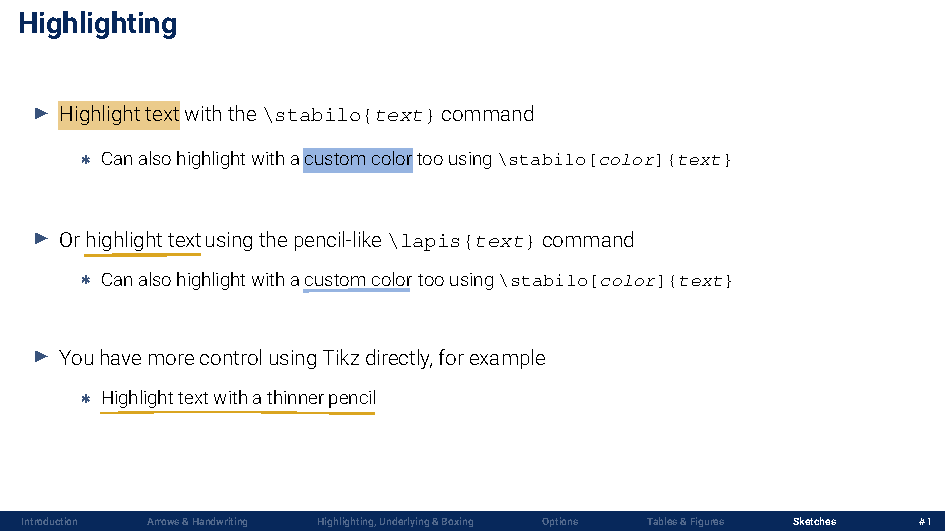
\includegraphics[width=\textwidth]{roboto}
        \end{minipage}
    \end{center}
\end{frame}
%.......................................................
\begin{flushleft}
    \underline{\textbf{Notes}}\setlength{\parskip}{.15cm}\notesize\newline\par
\end{flushleft}

%=============================================================
\begin{frame}
    {Theme's options}
    \begin{itemize}
        \item Set \texttt{cabin} option for cabin font
    \end{itemize}
    \begin{center}
        \begin{minipage}[b]{.6\textwidth}
            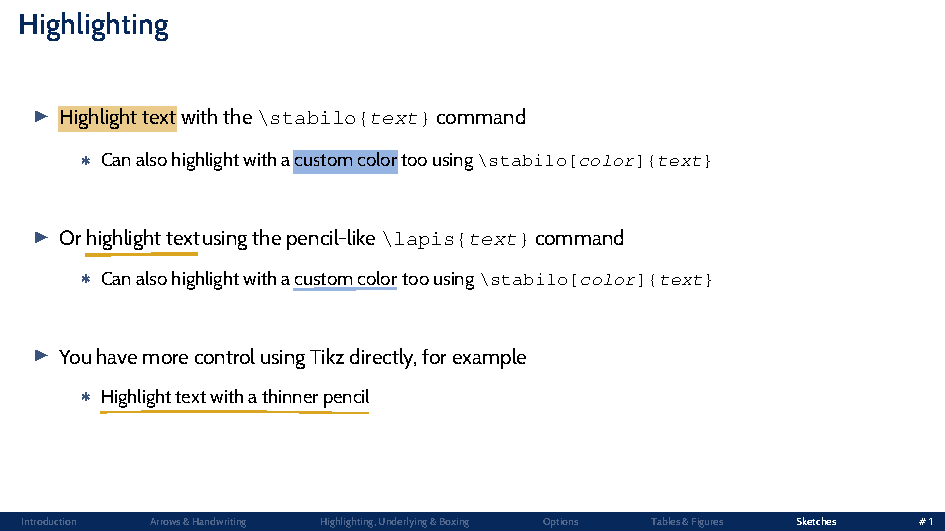
\includegraphics[width=\textwidth]{cabin}
        \end{minipage}
    \end{center}
\end{frame}
%.......................................................
\begin{flushleft}
    \underline{\textbf{Notes}}\setlength{\parskip}{.15cm}\notesize\newline\par
\end{flushleft}

%=============================================================
\begin{frame}
    {Theme's options}
    \begin{itemize}
        \item Set \texttt{night} option for dark scheme 
    \end{itemize}
    \begin{center}
        \begin{minipage}[b]{.6\textwidth}
            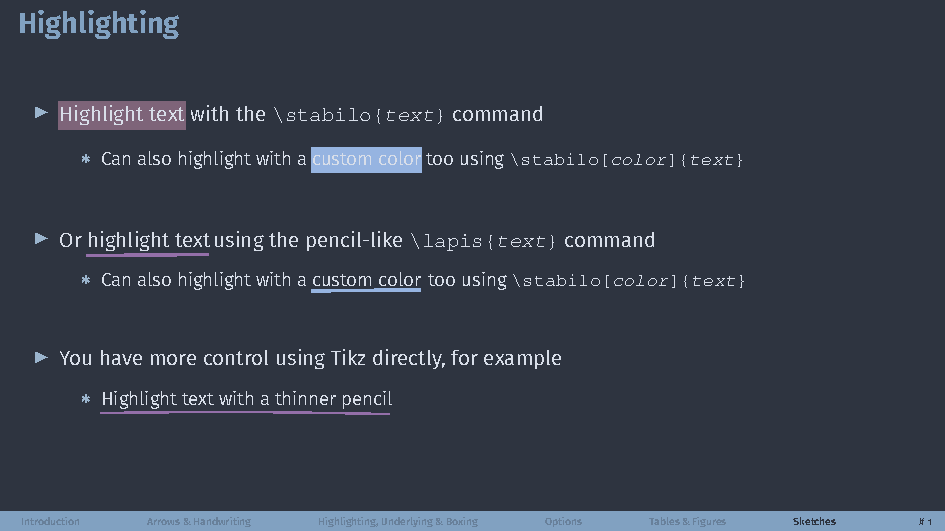
\includegraphics[width=\textwidth]{night}
        \end{minipage}
    \end{center}
\end{frame}
%.......................................................
\begin{flushleft}
    \underline{\textbf{Notes}}\setlength{\parskip}{.15cm}\notesize\newline\par
\end{flushleft}

%=============================================================
\begin{frame}
    {Theme's options}
    \begin{itemize}
        \item Set \texttt{red} option for red fonts
    \end{itemize}
    \begin{center}
        \begin{minipage}[b]{.6\textwidth}
            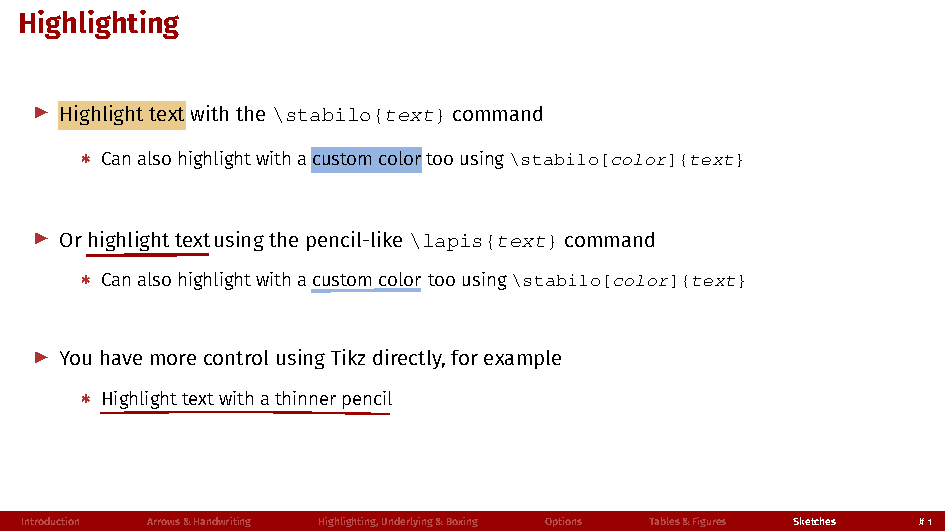
\includegraphics[width=\textwidth]{red}
        \end{minipage}
    \end{center}
\end{frame}
%.......................................................
\begin{flushleft}
    \underline{\textbf{Notes}}\setlength{\parskip}{.15cm}\notesize\newline\par
\end{flushleft}

%=============================================================
\begin{frame}
    {Theme's options}
    \begin{itemize}
        \item Set \texttt{3to2} option for 3 x 2 format 
    \end{itemize}
    \begin{center}
        \begin{minipage}[b]{.5\textwidth}
            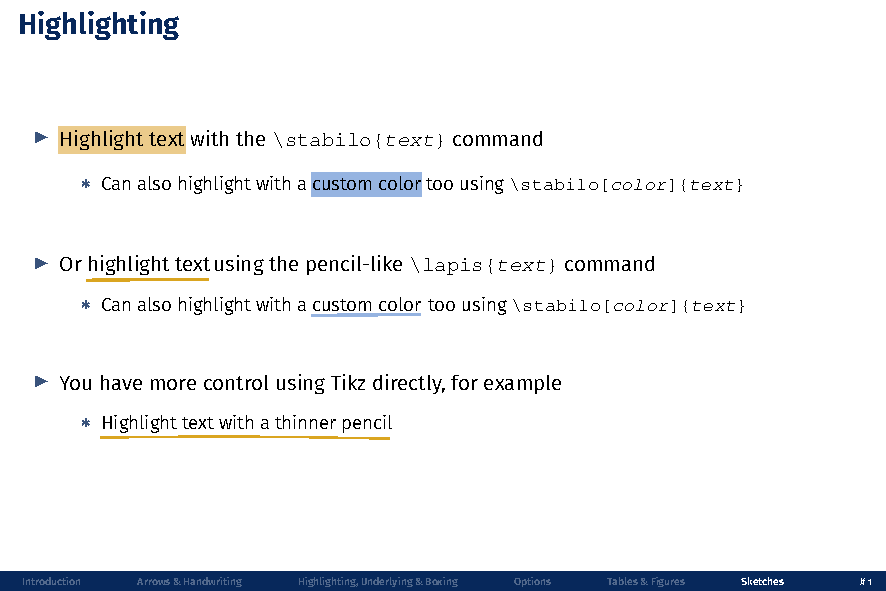
\includegraphics[width=\textwidth]{3to2}
        \end{minipage}
    \end{center}
\end{frame}
%.......................................................
\begin{flushleft}
    \underline{\textbf{Notes}}\setlength{\parskip}{.15cm}\notesize\newline\par
\end{flushleft}

%=============================================================
\begin{frame}
    {Theme's options}
    \begin{itemize}
        \item Set \texttt{shownotes} to show notes and \texttt{handout2x1} produce 2x1 handouts
    \end{itemize}
    \begin{center}
        \begin{minipage}[b]{.3\textwidth}
            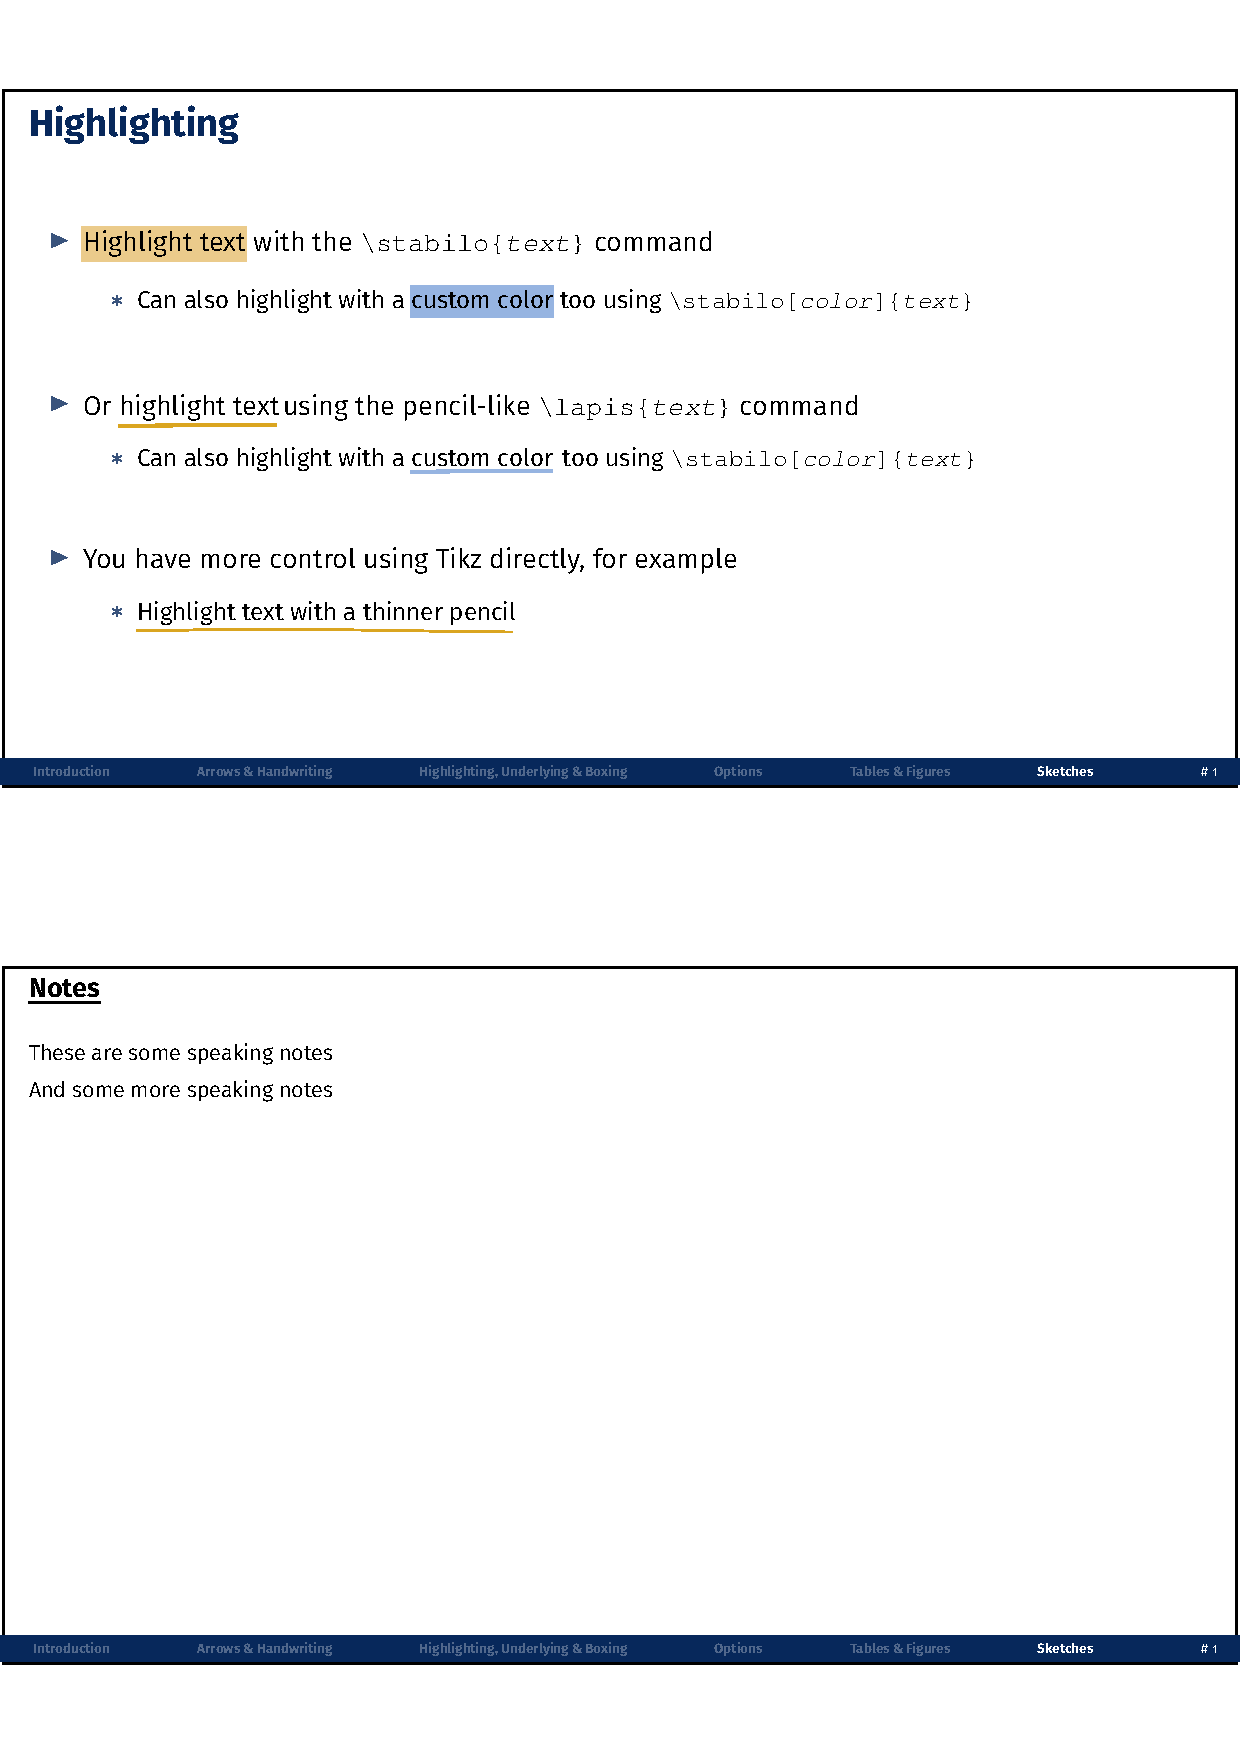
\includegraphics[width=\textwidth]{shownotes_handout}
        \end{minipage}
    \end{center}
\end{frame}
%.......................................................
\begin{flushleft}
    \underline{\textbf{Notes}}\setlength{\parskip}{.15cm}\notesize\newline\par
\end{flushleft}

%=============================================================
\begin{frame}
    {Theme's options}
    \begin{itemize}
        \item Set \texttt{onesec} to show only one section at the time in footline
    \end{itemize}
    \begin{center}
        \begin{minipage}[b]{.6\textwidth}
            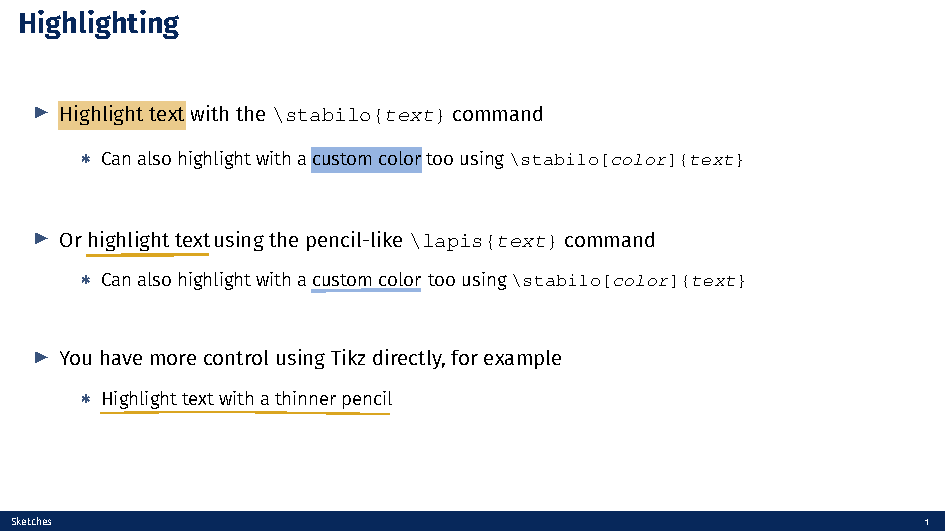
\includegraphics[width=\textwidth]{onesec}
        \end{minipage}
    \end{center}
\end{frame}
%.......................................................
\begin{flushleft}
    \underline{\textbf{Notes}}\setlength{\parskip}{.15cm}\notesize\newline\par
\end{flushleft}

%=============================================================
\section{Tables \& Figures}
\begin{frame}
    \begin{eqnarray*}
        &\text{{\huge \textbf{Tables \& Figures}}}\\
    \end{eqnarray*}
\end{frame}
%.......................................................
\begin{flushleft}
    \underline{\textbf{Notes}}\setlength{\parskip}{.15cm}\notesize\newline\par
\end{flushleft}

%=============================================================
\begin{frame}
    {Tables}
    \begin{itemize}
        \item This is a table using the \texttt{minipage} and \texttt{tabularx} commands
    \end{itemize}
    \begin{table}[th]
        \centering%
        \begin{minipage}[b]{.5\textwidth}
            \vspace{.2cm}\tablesize
            \begin{tabularx}{\textwidth}{lY}
                \toprule
                Dep. Variable: spread ($\Delta cs_{ij}$) 	& (1)\\
                \midrule
                & {Baseline Specification} \\
                \midrule
                \rowcolor{gray!10} Coeff. ($\beta_1$) 		&  21.15*** \\
                &   (7.35) \\
                \midrule
                \rowcolor{gray!10} Double clustering 		& Yes \\
                Time-sector FE 												& No \\
                \rowcolor{gray!10} R-squared 					& 0.034 \\
                Observations 												& 285,794 \\\bottomrule
            \end{tabularx}\vspace{.2cm}\newline
            \tiny{{\scshape Note.} Standard errors (reported in parentheses) are clustered two-way, at the firm level and time level. The asterisks denote statistical significance (*** for $p<0.01$, ** for $p<0.05$, * for $p<0.1$).\newline}%
            \label{tab:label2}%
        \end{minipage}
    \end{table}
\end{frame}
%.......................................................
\begin{flushleft}
    \underline{\textbf{Notes}}\setlength{\parskip}{.15cm}\notesize\newline\par
\end{flushleft}

%=============================================================
\begin{frame}
    {Tables}
    \begin{itemize}
        \item Control opacity of columns specifying alignment \texttt{S} within the \texttt{tabularx} command 
    \end{itemize}
    \begin{table}[th]
        \centering%
        \begin{minipage}[b]{.5\textwidth}
            \vspace{.2cm}\tablesize
            \begin{tabularx}{\textwidth}{lS}
                \toprule
                Dep. Variable: spread ($\Delta cs_{ij}$) 	& (1)\\
                \midrule
                & {Baseline Specification} \\
                \midrule
                \rowcolor{gray!10} Coeff. ($\beta_1$) 		&  21.15*** \\
                &   (7.35) \\
                \midrule
                \rowcolor{gray!10} Double clustering 		& Yes \\
                Time-sector FE 												& No \\
                \rowcolor{gray!10} R-squared 					& 0.034 \\
                Observations 												& 285,794 \\\bottomrule
            \end{tabularx}\vspace{.2cm}\newline
            \tiny{{\scshape Note.} Standard errors (reported in parentheses) are clustered two-way, at the firm level and time level. The asterisks denote statistical significance (*** for $p<0.01$, ** for $p<0.05$, * for $p<0.1$).\newline}%
            \label{tab:label3}%
        \end{minipage}
    \end{table}
\end{frame}
%.......................................................
\begin{flushleft}
    \underline{\textbf{Notes}}\setlength{\parskip}{.15cm}\notesize\newline\par
\end{flushleft}

%=============================================================
\begin{frame}
    {Tables}
    \begin{itemize}
        \item Control the width of the table with the \texttt{minipage} command \medskip
        \item If the table is not wide enough, the text (from column 2 onward) is automatically spread on multiple lines
    \end{itemize}
    \begin{table}[th]
        \centering%
        \begin{minipage}[b]{.4\textwidth}
            \vspace{.2cm}\tablesize
            \begin{tabularx}{\textwidth}{lY}
                \toprule
                Dep. Variable: spread ($\Delta cs_{ij}$) 	& (1)\\
                \midrule
                & {Baseline Specification} \\
                \midrule
                \rowcolor{gray!10} Coeff. ($\beta_1$) 		&  21.15*** \\
                &   (7.35) \\
                \midrule
                \rowcolor{gray!10} Double clustering 		& Yes \\
                Time-sector FE 												& No \\
                \rowcolor{gray!10} R-squared 					& 0.034 \\
                Observations 												& 285,794 \\\bottomrule
            \end{tabularx}\vspace{.2cm}\newline
            \tiny{{\scshape Note.} Standard errors (reported in parentheses) are clustered two-way, at the firm level and time level. The asterisks denote statistical significance (*** for $p<0.01$, ** for $p<0.05$, * for $p<0.1$).\newline}%
            \label{tab:label4}%
        \end{minipage}
    \end{table}
\end{frame}
%.......................................................
\begin{flushleft}
    \underline{\textbf{Notes}}\setlength{\parskip}{.15cm}\notesize\newline\par
\end{flushleft}

%=============================================================
\begin{frame}
    {Figures}
    \begin{itemize}
        \item This is a figure using the \texttt{minipage} and \texttt{includegraphics} commands
    \end{itemize}
    \begin{center}
        \begin{minipage}[b]{.6\textwidth}
            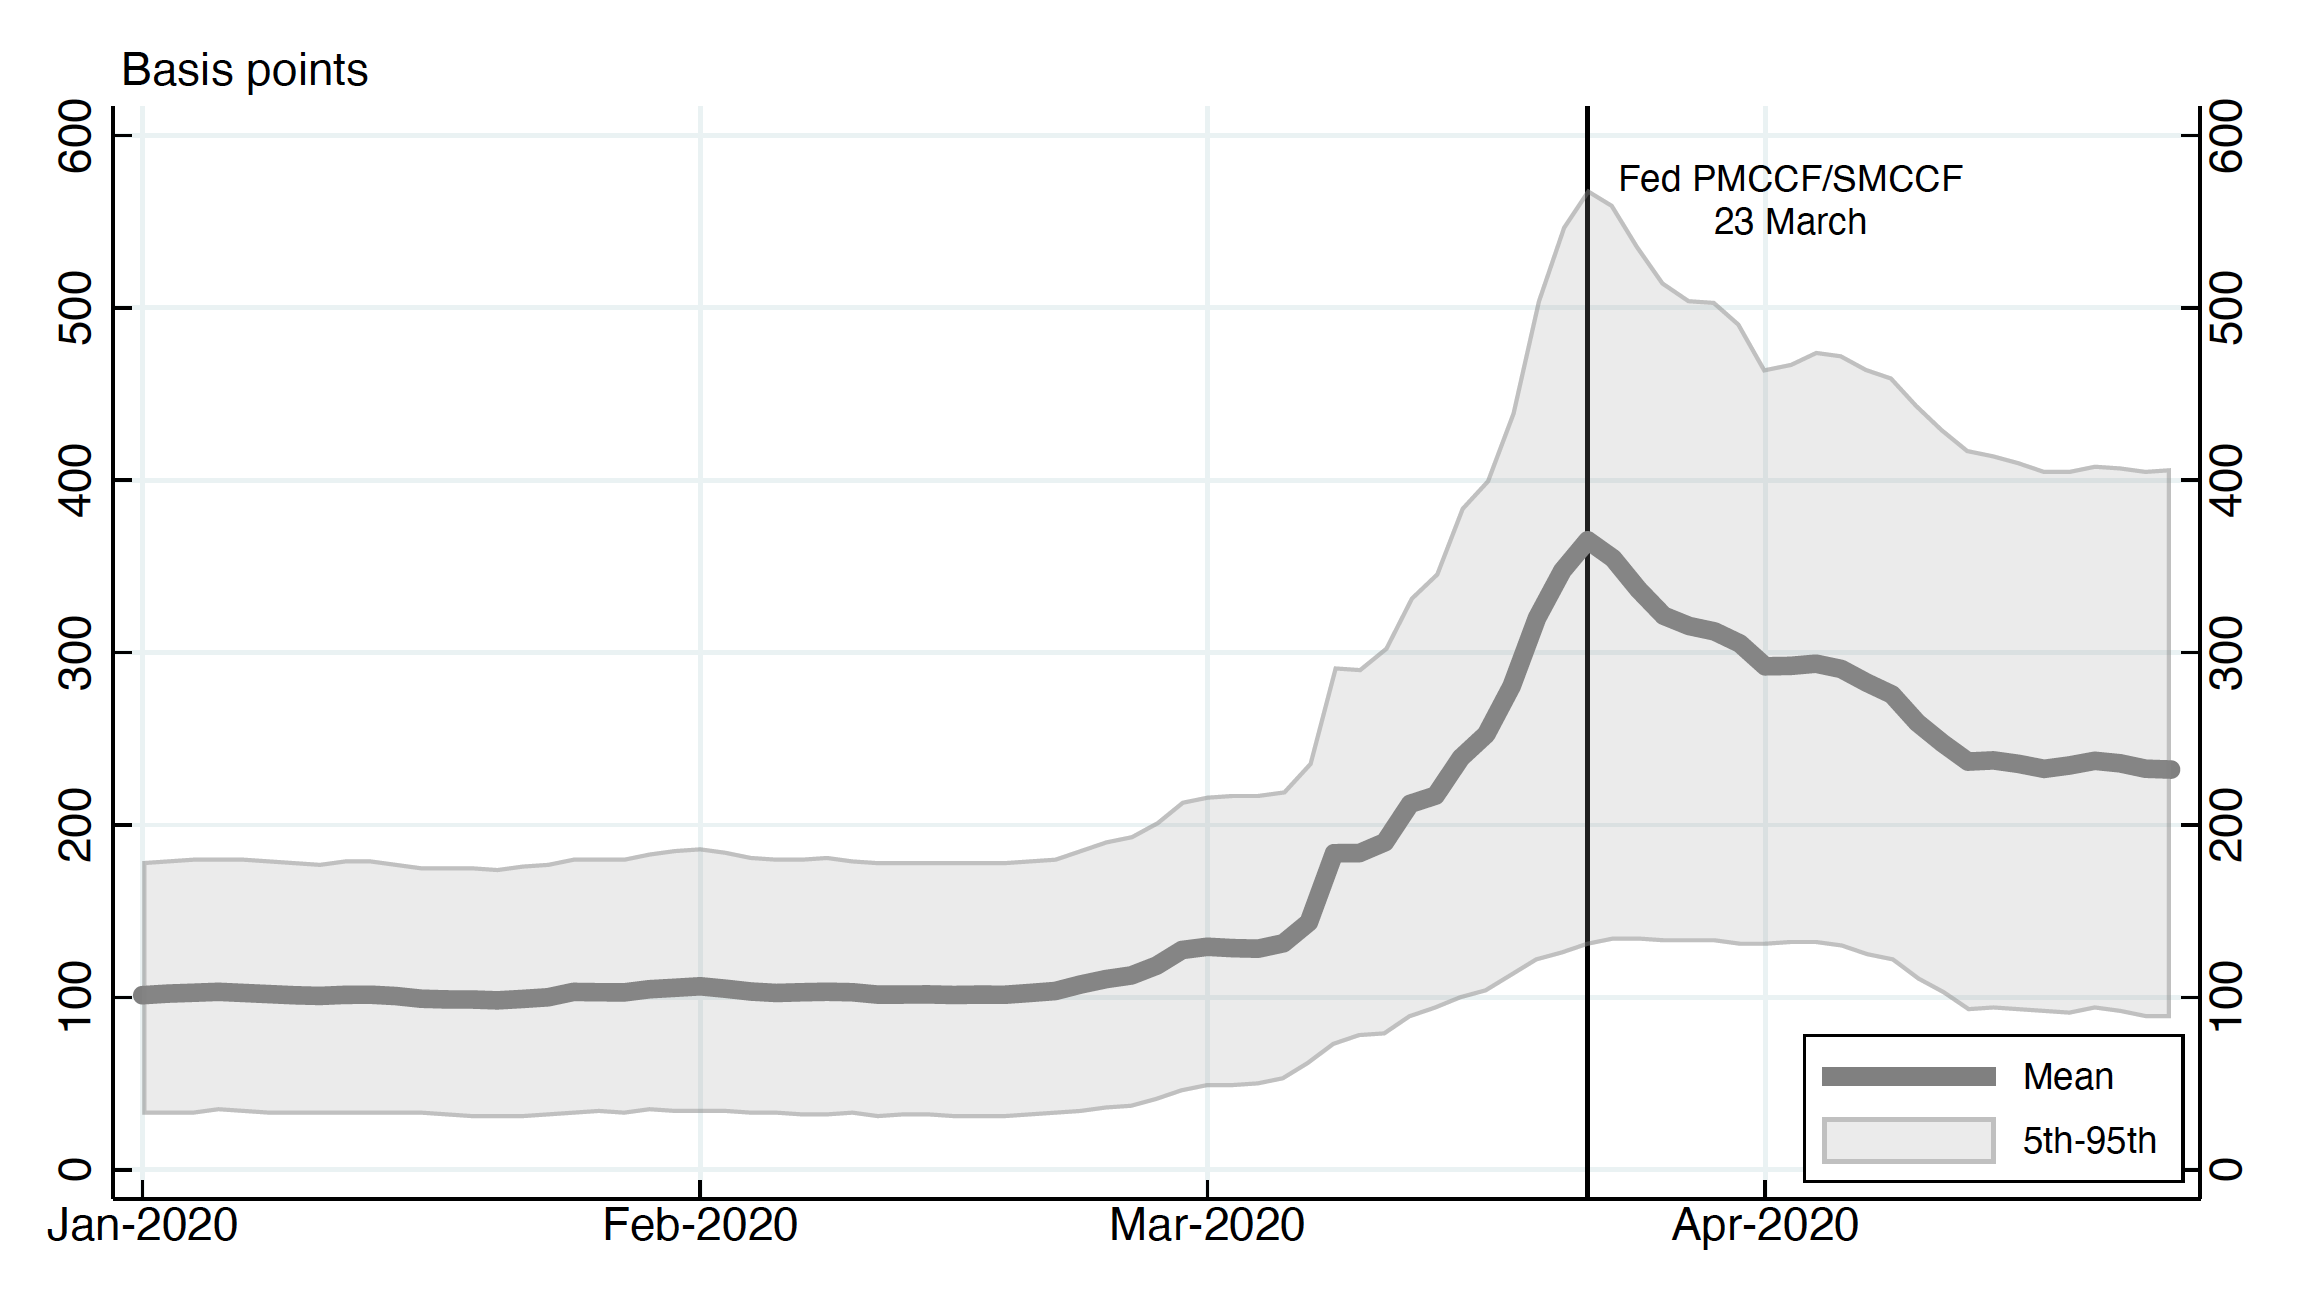
\includegraphics[width=\textwidth]{figure}\\
            \tiny{{\scshape Note}. \ Global average of investment grade corporate bond spreads (option-adjusted) weighted by bonds face value, together with 5th and 95th percentile of the full distribution. Source: ICE BoA ML.}
        \end{minipage}
    \end{center}
\end{frame}
%.......................................................
\begin{flushleft}
    \underline{\textbf{Notes}}\setlength{\parskip}{.15cm}\notesize\newline\par
\end{flushleft}


%=============================================================
\section{Sketches \& Bubbles}
\begin{frame}
    \begin{eqnarray*}
        &\text{{\huge \textbf{Sketches \& Bubbles}}}\\
    \end{eqnarray*}
\end{frame}
%.......................................................
\begin{flushleft}
    \underline{\textbf{Notes}}\setlength{\parskip}{.15cm}\notesize\newline\par
\end{flushleft}

%=============================================================
\begin{frame}{Sketch of a model}
    \begin{center}
        \begin{tikzpicture}
            % HOME
            %--------------
            % Home Banks
            \node[fill=title!70,text=white,rounded corners,inner sep=1ex,font=\bfseries,xshift=0cm,yshift=0cm] (Bank) {Home Banks};
            % Home Firm
            \node[fill=title!70,text=white,rounded corners,inner sep=1ex,font=\bfseries,xshift=+5.5cm,yshift=0cm] (Hfirm) {Home Non-financial Firms};
            % Home Households
            \node[fill=title!70,text=white,rounded corners,inner sep=1ex,font=\bfseries,xshift=-3.5cm,yshift=-3cm] (Hhh) {Home Households};
            % Arrows 
            \draw[arrow,black,->,very thick] ([xshift=0.2cm]Bank.east) to ([xshift=-0.2cm]Hfirm.west);
            \draw[snake,black,->,very thick] ([xshift=0.2cm]Hhh.east) to [bend right] ([yshift=-0.2cm]Bank.south);
            % Labels
            \draw[] (1.1cm,-1.6cm) node[anchor=north,opacity=1,] {\small \hand LC deposits};
            \draw[title!70] (1.1cm,-2cm) node[anchor=north,opacity=1,] {\small \hand \footnotesize{Agency friction}};
            \draw[] (2.1cm,.6cm) node[anchor=north,opacity=1,] {\small \hand Securities};
            % US
            %--------------
            % US Household
            \node[fill=title!70,text=white,rounded corners,inner sep=1ex,font=\bfseries,xshift=-3.5cm,yshift=3cm] (Fhh) {US Household};
            % Arrows 
            \draw[snake,black,->,very thick] ([xshift=0.2cm]Fhh.east) to [bend left] ([yshift=0.2cm]Bank.north);
            % Labels
            \draw[] (-2.3cm,2.4cm) node[anchor=north,opacity=1,] {\small \hand USD deposits};
            \draw[title!70] (-2.3cm,2cm) node[anchor=north,opacity=1,] {\hand \footnotesize{More severe}};
            \draw[title!70] (-2.3cm,1.7cm) node[anchor=north,opacity=1,] {\hand \footnotesize{Agency friction}};
            % SWAP LINES
            %--------------
            % Fed
            \node[fill=title!70,text=white,rounded corners,inner sep=1ex,font=\bfseries,xshift=-5.5cm,yshift=1.5cm] (Fed) {Fed};
            % Home CB
            \node[fill=title!70,text=white,rounded corners,inner sep=1ex,font=\bfseries,xshift=-4.5cm,yshift=-1cm] (CB) {Home Central Bank};
            % Arrows 
            \draw[arrow,black,<->,very thick] ([xshift=0cm]Fed.south west) to [bend right] ([xshift=-0cm]CB.north west);
            \draw[arrow,black,->,very thick] ([xshift=0.2cm]CB.east) to [bend right] ([xshift=-0cm]Bank.south west);
            % Labels
            \draw[] (-5.3cm,0.5cm) node[anchor=north,opacity=1] {\small \hand Swap line};
            \draw[] (-2cm,0.1cm) node[anchor=north,opacity=1] {\small \hand USD};
            \draw[] (-2cm,-0.2cm) node[anchor=north,opacity=1] {\small \hand funds};
        \end{tikzpicture}
    \end{center}
\end{frame}
%.......................................................
\begin{flushleft}
    \underline{\textbf{Notes}}\setlength{\parskip}{.15cm}\notesize\newline\par
\end{flushleft}

%=============================================================
\begin{frame}{Sketch of demand and supply}
    \begin{center}
        \begin{tikzpicture}[scale=1.9, important line/.style={thick}, dashed line/.style={dashed, thin}, every node/.style={color=black}, dot/.style={circle,fill=black,minimum size=5.5pt,inner sep=0pt,outer sep=-1pt}]
            % Axes
            \draw[thick, ->, >=stealth', line join=miter,<->](3,0) 
            node(xline)[below,xshift=-2.5cm, yshift=-.1cm] {\small{\hand Capital $(K)$}} -| (0,2.5) 
            node(yline)[above,rotate=90,xshift=-2.5cm, yshift=1cm] {\small{\hand Credit Spread $\left(R^B/R\right)$}};
            % Demand
            \draw[scale=0.5,domain=1.7:2.9,smooth,variable=\x,thick,gray,opacity=0.6]  plot ({\x}, {3-4*ln(\x-1)}) node[right, opacity=1] {\footnotesize{\hand Demand $(K^D_{j,\ell})$}};
            % Supply LOW
            \draw[scale=0.5,domain=0:1.2,smooth,variable=\x,thick,red] plot ({\x},  {1});
            \node[label=left: $1$] at (0,0.5) (int1) {};	
            \draw[scale=0.5,domain=1.2:2.35,smooth,variable=\x,thick,red] plot ({\x},  {1+2*(\x-1.2)^2}) node[right] {\footnotesize{\hand Supply $(K^S_{j,\ell})$}};
            % Equilibria
            \node[circle,draw=black, fill=red,inner sep=1.25pt] at (1.05,1.3) (int1) {};
            \node[label=\footnotesize  $\mathcal{A}_\ell$] at (0.89,1.12) (int1) {};
        \end{tikzpicture}
        \begin{tikzpicture}[scale=1.9, important line/.style={thick}, dashed line/.style={dashed, thin}, every node/.style={color=black}, dot/.style={circle,fill=black,minimum size=5.5pt,inner sep=0pt,outer sep=-1pt}]
            % Axes
            \draw[thick, ->, >=stealth', line join=miter,<->](3,0) 
            node(xline)[below,xshift=-2.5cm, yshift=-.1cm] {\small{\hand Capital $(K)$}} -| (0,2.5);
            % Demand
            \draw[scale=0.5,domain=1.7:2.9,smooth,variable=\x,thick,gray,opacity=0.6]  plot ({\x}, {3-4*ln(\x-1)}) node[right, opacity=1] {\footnotesize{\hand Demand $(K^D_{j,h})$}};
            % Supply HIGH 
            \draw[scale=0.5,domain=0:2,smooth,variable=\x,thick,main] plot ({\x},  {1});
            \node[label=left: $1$] at (0,0.5) (int1) {};	
            \draw[scale=0.5,domain=2:3.5,smooth,variable=\x,thick,main] plot  ({\x}, {1+0.6*(\x-2)^2}) node[right] {\footnotesize{\hand Supply $(K^S_{j,h})$}};
            % Equilibria
            \node[circle,draw=black, fill=main,inner sep=1.25pt] at (1.29,0.6) (int1) {};
            \node[label=\footnotesize  $\mathcal{A}_h$] at (1.45,0.35) (int1) {};
        \end{tikzpicture}
    \end{center}
\end{frame}
%.......................................................
\begin{flushleft}
    \underline{\textbf{Notes}}\setlength{\parskip}{.15cm}\notesize\newline\par
\end{flushleft}

%=============================================================
\begin{frame}
    {Bubbles}
    \begin{itemize}
        \item The theme allows to create bubbles with the \texttt{\textbackslash NB} command in combination with the \texttt{minipage} environment \bigskip
    \end{itemize}
    \begin{center}
        \begin{minipage}{.4\textwidth}
            \NB{This is a small bubble}
        \end{minipage}
    \end{center}
    \begin{center}
        \begin{minipage}{.6\textwidth}
            \NB{This is a large bubble.\\ With two lines}
        \end{minipage}
    \end{center}
    \begin{center}
        \begin{minipage}{.8\textwidth}
            \NB{This is a larger bubble with bullets:
                \begin{itemize}
                    \item Uno
                    \item Dos
                    \item Tres 
            \end{itemize}}
        \end{minipage}
    \end{center}
\end{frame}
%.......................................................
\begin{flushleft}
    \underline{\textbf{Notes}}\setlength{\parskip}{.15cm}\notesize\newline\par
\end{flushleft}


%=============================================================
\section{Misc}
\begin{frame}
    \begin{eqnarray*}
        &\text{{\huge \textbf{Miscellaneous}}}\\
    \end{eqnarray*}
\end{frame}
%.......................................................
\begin{flushleft}
    \underline{\textbf{Notes}}\setlength{\parskip}{.15cm}\notesize\newline\par
\end{flushleft}

%=============================================================
\begin{frame}[fragile]
    {Verbatim \& Code}
    \begin{itemize}
        \item The command \texttt{\textbackslash jverb\{...\}} allows to write inline \jverb{verbatim text} \vs{4} 
        \item And  the command \texttt{\textbackslash begin\{jVerb\}} can be used for a verbatim box \vs{1} 
        \begin{jVerb}
        >> disp(VAR_sigma)
        0.2891    0.0782
        0.0782    0.1473
        \end{jVerb}
        \item \jcode{Code} can be added with the command \texttt{\textbackslash jcode\{...\}} (does not support verbatim) \vs{4} 
        \item Code boxes can be added with the command \texttt{\textbackslash jCode\{...\}} 
        \jCode{%
            \hspace{1mm}\textcolor{matlabgreen}{\% Compute HD}\\
            \hspace{1mm}[HD, VAR] = VARhd(VAR,VARopt); \\
        }
        \item All commands in this page require \jverb{\begin{frame}[fragile]}
    \end{itemize}
\end{frame}
%.......................................................
\begin{flushleft}
    \underline{\textbf{Notes}}\setlength{\parskip}{.15cm}\notesize\newline\par
\end{flushleft}

%=============================================================
\begin{frame}
    {Change Margins}
    \begin{itemize}
        \item This is a tight margin:  \vs{3}
        \begin{changemargin}{2cm}{2cm}
            Lorem ipsum dolor sit amet, consectetur adipiscing elit, sed do eiusmod tempor incididunt ut labore et dolore magna aliqua. Ut enim ad minim veniam, quis nostrud exercitation ullamco laboris nisi ut aliquip ex ea commodo consequat. 
        \end{changemargin}\bigskip
        \item This is a wide margin:  \vs{3}
        \begin{changemargin}{-0.4cm}{-0.4cm}
            Lorem ipsum dolor sit amet, consectetur adipiscing elit, sed do eiusmod tempor incididunt ut labore et dolore magna aliqua. Ut enim ad minim veniam, quis nostrud exercitation ullamco laboris nisi ut aliquip ex ea commodo consequat. 
        \end{changemargin}
    \end{itemize}
\end{frame}
%.......................................................
\begin{flushleft}
    \underline{\textbf{Notes}}\setlength{\parskip}{.15cm}\notesize\newline\par
\end{flushleft}

    
    
    
    
\end{document}


